\documentclass[hyperref={pdfpagelabels=false}]{beamer}
\graphicspath{{Graph/}{./}} % Specifies where to look for included images (trailing slash required)
\usepackage{booktabs} % Allows the use of \toprule, \midrule and \bottomrule for better rules in tables
\usepackage{calligra} % Font for wordart
\usepackage{appendixnumberbeamer} % If you want a separate slide counter for your appendix
\usepackage{fnpct} % Eliminate the unwanted space before the footnote mark
\usepackage{listings} % For code display


%---------------------------------------------------------
%	CITATIONS / REFERENCES
%---------------------------------------------------------
\usepackage[style=authoryear]{biblatex}
\addbibresource{bib.bib}
%\bibliographystyle{apalike}



%---------------------------------------------------------
%	SELECT THEME & COLORS
%---------------------------------------------------------
\usetheme{Madrid}
\definecolor{MonashBlue}{RGB}{0, 99, 167}
\definecolor{Orange}{RGB}{204, 89, 0}

\setbeamercolor*{structure}{bg=MonashBlue, fg=MonashBlue}
% Title block and bottom right box color
\setbeamercolor*{palette primary}{use=structure, fg=white,bg=MonashBlue}
% Bottom left box and bar between title & top bubbles
\setbeamercolor*{palette secondary}{use=structure, fg=MonashBlue, bg=white}
% Probably not used
\setbeamercolor*{palette tertiary}{use=structure, fg=white, bg=MonashBlue} 

% Title of each slide
\setbeamercolor{frametitle}{bg=MonashBlue, fg=white}
\setbeamercolor*{titlelike}{parent=palette primary}


%%% Headline and Central Footer %%%
% You can change the theme back and forth for each frame

% Theme II - gold head, gold foot (as shown in the title frame)
    \setbeamercolor{section in head/foot}{fg=white, bg=Orange}
    \setbeamercolor{headline}{fg=white, bg=Orange}



%%% Specific Colors %%%
\setbeamercolor{item projected}{bg=Orange}
\setbeamertemplate{enumerate items}{bg=Orange}

\setbeamercolor{itemize item}{fg=Orange}
\setbeamercolor{itemize subitem}{fg=Orange}

\setbeamercolor{button}{bg=Orange}

%%% Edits ONLY the TOC slide %%%
\setbeamercolor{section in toc}{fg=black}
\setbeamercolor{subsection in toc}{fg=black}

%%% Block Colors %%%
% Standard block
    \setbeamercolor{block title}{bg=Orange, fg=white}
    \setbeamercolor{block body}{bg=Orange!20}
% Alerted block
    \setbeamercolor{block title alerted}{bg=orange, fg=white}
    \setbeamercolor{block body alerted}{bg=orange!10}
% Example block
    \setbeamercolor{block title example}{bg=MonashBlue, fg=white}
    \setbeamercolor{block body example}{bg=MonashBlue!10}

%---------------------------------------------------------
%	SELECT THE FONT THEME & FONTS
%---------------------------------------------------------
\usefonttheme{default} % Typeset using the default sans serif font
\usepackage{palatino} % Use the Palatino font for serif text
\usepackage[default]{opensans} % Use the Open Sans font for sans serif text
\useinnertheme{circles}

%---------------------------------------------------------
%	SELECT THE OUTER THEME
%---------------------------------------------------------

% \useoutertheme{default}
% \useoutertheme{miniframes}
% \useoutertheme{infolines}
% \useoutertheme{smoothbars}
% \useoutertheme{sidebar}
 \useoutertheme{split}
% \useoutertheme{shadow}
% \useoutertheme{tree}
% \useoutertheme{smoothtree}

%---------------------------------------------------------
%	PRESENTATION INFORMATION
%---------------------------------------------------------

\title[Revisiting Forecast Combination Puzzle]{Revisiting Forecast Combination Puzzle}
% Click the middle footer can switch between the first and last numbered frame
\subtitle{An Empirical Study}
\medskip
\author[Honours Preliminary Presentation]{\Large{XIEFEI (SAPPHIRE) LI}}
\institute[]{Department of Econometrics and Business Statistics \\ \medskip
\textit{xlii0145@student.monash.edu} \\ \bigskip
\text{\small{Supervisor: David T. Frazier}}
}
\date[May 2023]

\logo{
\includegraphics[width=2.5cm]{Monash.png}}

%---------------------------------------------------------
%	CODE DISPLAY
%---------------------------------------------------------
\lstset{
    basicstyle=\ttfamily\small,
    keywordstyle=\bfseries\color{blue},
    emphstyle=\ttfamily\color{red},   
    stringstyle=\color{green},
    numbers=left,
    numberstyle=\small\color{gray},
    rulesepcolor=\color{red!20!green!20!blue!20},
    frame=shadowbox,
    xleftmargin=1cm,
    xrightmargin=1cm,
}

%---------------------------------------------------------
%	EXTRA SETTINGS
%---------------------------------------------------------

% Clear warnings related to \translate
%     https://github.com/josephwright/beamer/issues/449
\pdfstringdefDisableCommands{
    \def\translate#1{#1}
}

% Adjust header height
\setbeamertemplate{headline}{
    \nointerlineskip
    \begin{beamercolorbox}[wd=\paperwidth,ht=7.0ex]{headline}
        \insertnavigation{\paperwidth}\vspace*{2.0ex}
    \end{beamercolorbox}
}

% Disable navigation symbols
\setbeamertemplate{navigation symbols}{}
\setbeamersize
{
    text margin left=1cm,
    text margin right=1cm
}

%---------------------------------------------------------
%   DOCUMENT BEGINS
%---------------------------------------------------------
\begin{document}

%---------------------------------------------------------
%	TITLE SLIDE
%---------------------------------------------------------
\section{}

\begin{frame}
\titlepage % Output the title slide, automatically created using the text entered in the PRESENTATION INFORMATION block above
\end{frame}

% Clear background
\usebackgroundtemplate{}



\setbeamercolor{section in head/foot}{fg=Orange, bg=white}
\setbeamercolor{headline}{fg=Orange, bg=white}

\section{Motivation}

\logo{}

\begin{frame}{Forecast combination - point and density}

    Combining multiple forecasts can dramatically improve the accuracy of the forecast (\cite{BG69}).
    
    \vspace{5mm}

    
    Point Forecast Combination 
    \[\hat y_t = \omega \ \hat y_{1t} + (1-\omega) \ \hat y_{2t}\]

    Density Forecast Combination
    \[ \hat f(y_t) = \omega \ \hat f_1(y_t) + (1-\omega) \hat f_2(y_t)\]

\end{frame}


\begin{frame}{Forecast combination puzzle}

\begin{columns}[t]
    \begin{column}{0.5\textwidth}
        \centering
        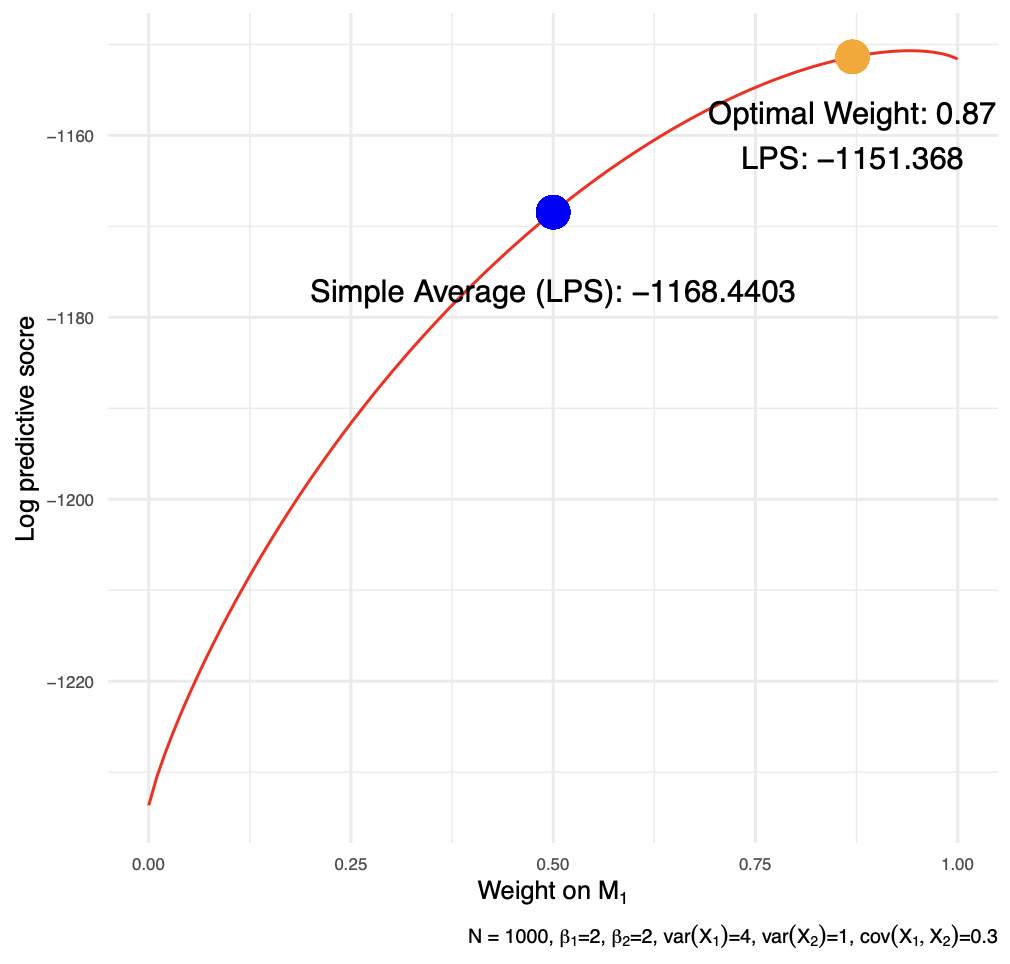
\includegraphics[width=6cm]{Graph/Ex1.png}
    \end{column}
    
    \begin{column}{0.5\textwidth}
        \centering
        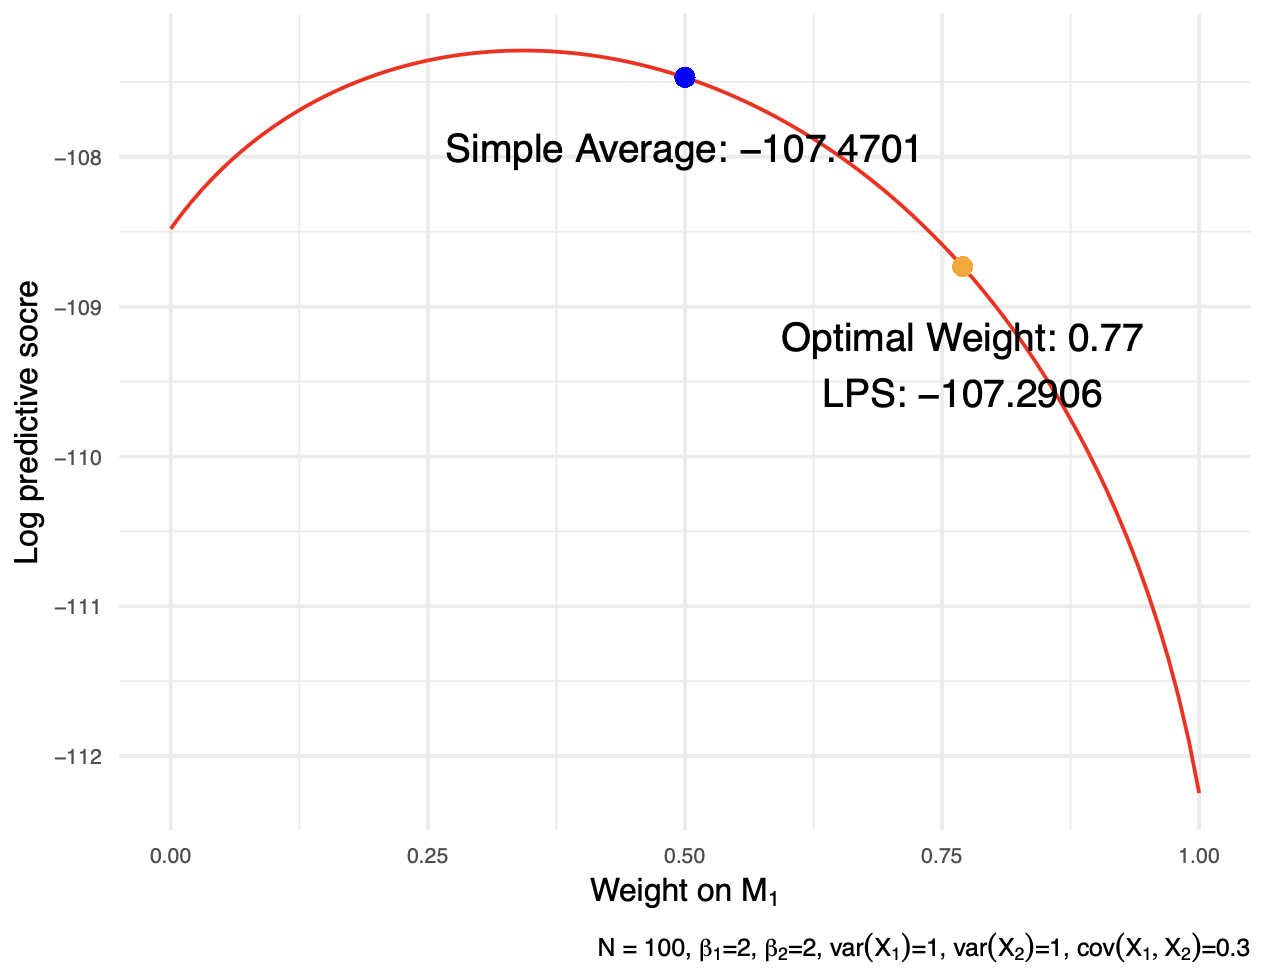
\includegraphics[width=6cm]{Graph/Ex2.png}
    \end{column}
    \end{columns}

    \vspace{-6mm}
    
    \begin{columns}[t]
    \begin{column}{0.5\textwidth}
        \begin{alertblock}{}
        \centering
        \tikz{\fill[orange] circle (3pt);} \ Complicated Weighting Schemes
        \end{alertblock}
    \end{column}
    
    \begin{column}{0.5\textwidth}
        \begin{exampleblock}{}
        \centering
        \tikz{\fill[blue] circle (3pt);} \ Simple Averaging
        / Equal Weights
        \end{exampleblock}
    \end{column}
    \end{columns}

\end{frame}



\begin{frame}{When should we expect the puzzle}

    In the linear regression context, the optimal weight $\hat\omega_{opt}$ has a closed-form expression when using the Mean Squared Error (MSE) weighting scheme.
    
    
    \[\hat\omega_{opt} \overset{p}{\to} \omega_\star = \frac{\alpha_1'\Sigma_{11}\alpha_1 - \alpha_1'\Sigma_{12}\alpha_2}{\alpha_1'\Sigma_{11}\alpha_1 - 2\alpha_1'\Sigma_{12}\alpha_2 + \alpha_2'\Sigma_{22}\alpha_2}\]


    The presence of the puzzle is tightly related to the coefficients and the variances of regressors in both proposed models.
    
    
    \[\omega_\star=\frac{1}{2} \Rightarrow \alpha_1'\Sigma_{11}\alpha_1 = \alpha_2'\Sigma_{22}\alpha_2\]

    In-sample performance

    
\end{frame}



\begin{frame}{Preliminary Conjecture}

    Consider a two-model combination.

    \begin{table}[ht]
    \centering
    \begin{tabular}{cccc}
                           &      & \multicolumn{2}{c}{$M_2$} \\
                           &      & Good       & Bad       \\
    \multirow{2}{*}{$M_1$} & Good & \alt<2>{\color{MonashBlue} $\surd$}{$\surd$}    & \alt<2>{\color{Orange} $?$}{$?$} \\
                           & Bad  & \alt<2>{\color{Orange} $?$}{$?$}        & \alt<2>{\color{MonashBlue} $\surd$}{$\surd$}
    \end{tabular}
    \label{tab:1}
    \caption{\footnotesize Initial conjecture on the presence of forecast combination puzzle}
    \end{table}
    
    The in-sample fit between two models in a relative sense may indicate the presence of the puzzle.


\end{frame}



\begin{frame}{Preliminary Conjecture}
\centering
\begin{tikzpicture}
    \draw[step=1cm,gray,very thin];
    \draw[thick,->] (0,0) -- (7,0);
    \draw[thick,->] (0,0) -- (0,5);
    \draw[thick,->] (0,0) -- (7,0) node[anchor=north west] {$M_1$ LogL};
    \draw[thick,->] (0,0) -- (0,5) node[anchor=south east] {$M_2$ LogL};
    
    \foreach \Point in {(1,1), (2,2), (3,3), (4,4)}{
    \node [MonashBlue] at \Point {$\surd$};}
    
    \foreach \Point in {(6,2), (5,1), (1,4), (2,5)}{
    \node [Orange] at \Point {$?$};}

    \foreach \Point/\PointLabel in {(6,2)/GB, (5,1)/GB, (1,4)/BG, (2,5)/BG}
        \draw[fill=Orange] \Point circle (0.0005) node[above right] {\color{Orange} \PointLabel};
\end{tikzpicture}

\end{frame}







\section{Aim}

\begin{frame}
    \frametitle{Research objectives}

    \begin{itemize}
        \item The determinants behind, and evidence for, the forecast combination puzzle in various settings, besides the time series domain \newline
        \item The veracity, and applicability, of a recently proposed solution to forecasting combination puzzle suggested in \cite{ZMFP22} and \cite{FZMP23}.
    \end{itemize}
    
\end{frame}



\section{Methodology}


\begin{frame}
\label{Figure}
	\frametitle{Forecast combination method}
		
        A linear combination of two predictive densities, $f(y_t)$, is constructed with two constituent predictive densities $f_1(y_t)$ and $f_2(y_t)$:
        
        \vspace{3mm}
        
        \begin{equation}
        f(y_t) = w \ f_1(y_t) + (1-w) \ f_2(y_t)
        \end{equation}  
        
        \vspace{5mm}
        
        where $w$ \footnote{\scriptsize{Through this construction, the sum of two weights is implied to be 1, which is necessary and sufficient for the combination to be a density function [\cite{GA11}].}} is the weight allocated to the first model. 
        
\end{frame}


\begin{frame}
\frametitle{Parameters Estimation}

The unknown parameters, $\theta_M$, of each model ($M$) are estimated by maximizing the log likelihood function of the conditional probability density over the in-sample period ($R$):

\begin{equation}
    \hat\theta_M = \text{argmax} \sum^R_{t=1} log f(y_t|M).
\end{equation}
 
\end{frame}

\begin{frame}{Log predictive score function}

Following \cite{GA11}, we measure the accuracy of density forecasts with the log predictive score function for each model, which is defined as:

\begin{equation}
LS = \sum^P_{h=1} log\ f(y_{\small{R+h}}| \mathcal{F}_{\small{R+h-1}}, \hat\theta_M, M)
\end{equation}

\vspace{5mm}
\scriptsize{where $P$ denotes the out-of-sample period and $h$ is the forecast horizon with $h>0$. $\mathcal{F}_{\small{R+h-1}}$ denotes all information available at time $R+h-1$, and we assume that the conditional mean and variance of the models are, up to unknown parameters, known at time $R+h-1$. }

\end{frame}

\begin{frame}{Weight Estimation}
    The weight ($w$) assigned to the first model will be estimated by maximizing the log predictive score function over the out-of-sample period:

\begin{multline}
\hat{w} = \text{argmax} \sum^P_{h=1}log\Big[w \ f_1(y_{\small{R+h}}|\mathcal{F}_{\small{R+h-1}}, \hat\theta_{M_1}, M_1) \\
 + (1-w) \ f_2(y_{\small{R+h}}|\mathcal{F}_{\small{R+h-1}}, \hat\theta_{M_2}, M_2)\Big]
\end{multline}

\end{frame}




\section{Preliminary Results}


\begin{frame}
    \frametitle{Model Specification I}
    
Data: Standard and Poor’s (S\&P) 500 index retrieved from the \cite{SP500}.

\vspace{2mm}

    \begin{itemize}
    \item ARIMA(1,1,1) model 
        \begin{equation*}
        log(y_t) = c + log(y_{t-1}) + \phi_1\big[log(y_{t-1})-log(y_{t-2})\big] + \epsilon_t + \theta_1\epsilon_{t-1}
        \end{equation*}
    \item ETS(M,N,N) model
        \begin{align*}
        y_t &= \ell_{t-1} (1+\epsilon_t) \\
        \ell_t &= \ell_{t-1} (1+\alpha \epsilon_t) \\
        \end{align*}
        \vspace{-1cm}
    \item ETS(M,A,N) model
        \begin{align*}
        y_t &= (\ell_{t-1} + b_{t-1} (1+\epsilon_t) \\
        \ell_t &= (\ell_{t-1} + b_{t-1}) (1+\alpha \epsilon_t) \\
        b_t &= b_{t-1} + \beta (\ell_{t-1} + b_{t-1})\epsilon_t \\
        \end{align*}
    \end{itemize}

\end{frame}

\begin{frame}
    \frametitle{Model Specification II}

    \begin{itemize}
    \item A linear regression model of the S\&P 500 with a trend regressor and errors follow an ARIMA(1,0,0) process. 
        \begin{align*}
        y_t &= \beta_0 + \beta_1 t + u_t \\
        u_t &= \phi_1 \epsilon_{t-1} + \epsilon_t
        \end{align*}

    \item A linear regression model of the natural logarithm of S\&P 500 with a trend regressor and errors follow an ARIMA(1,0,0) process. 
        \begin{align*}
        log(y_t) &= \beta_0 + \beta_1 t + u_t \\
        u_t &= \phi_1 \epsilon_{t-1} + \epsilon_t
        \end{align*}
    \end{itemize}

Error terms $\epsilon_t$ in each model are assumed to be independent and normally distributed with a zero mean and a constant variance.

\end{frame}



\begin{frame}
    \frametitle{Ten sets of two-model pools}

\begin{table}[ht]
  \centering
  \small
  \caption{Log predictive score of density forecasts combination under two-model pools}
  \scalebox{0.80}{
    \begin{tabular}{llllll}
    \toprule
          & ARIMA(1,1,1) & ETS(M,N,N) & ETS(M,A,N) &  LM (linear) &  LM (log) \\
    \midrule
    ARIMA(1,1,1) & \textit{-5911.1974} & -5839.3045 & -5842.7634 & -5911.1974 & -5894.1267 \\
    ETS(M,N,N) & 0.45  & \textit{-5883.9697} & -5881.7790 & -5883.9697 & -5858.6397 \\
    ETS(M,A,N) & 0.43  & 0.08  & \textit{-5881.7970} & -5881.7970 & -5859.7980 \\
     LM (linear) & 1     & 1     & 1     & \textit{-7532.1464} & -5918.5230 \\
     LM (log) & 0.56  & 0.65  & 0.67  & 0     & \textit{-5918.5230} \\
    \bottomrule
    \multicolumn{6}{l}{\footnotesize The diagonal entries contains individual log score.}\\
    \multicolumn{6}{l}{\footnotesize The log scores for combination pools are located above the diagonal.}\\
    \multicolumn{6}{l}{\footnotesize Entries below the diagonal show the estimated weight of the model in that column.}\\
    \end{tabular}
    }
  \label{tab:2}
\end{table}

\end{frame}




\begin{frame}
    \frametitle{Top 4 Combinations}

\begin{figure}[ht]
\centering
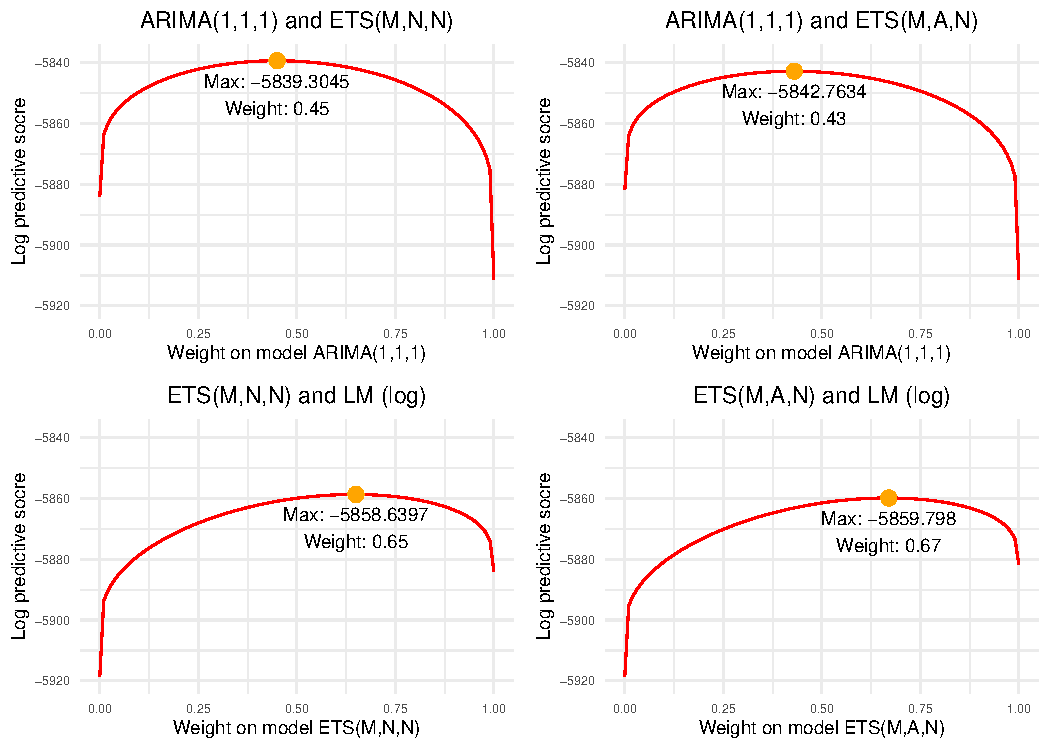
\includegraphics[width=9cm]{Graph/best4comb.pdf}\\
{\tiny{The top four log predictive scores of weighted two-model-pool combinations for S\&P 500 returns.}}
\end{figure}

\end{frame}




\section{Conclusion}

\begin{frame}
	\frametitle{Conclusion}
 
 Forecast combinations can deliver improved accuracy over single models, but are not necessarily superior to forecasts obtained from the equally weighted combination.

\end{frame}


\begin{frame}
	\frametitle{Timeline}
 
 \begin{table}[htbp]
  \centering
    \begin{tabular}{ll}
    Time  & Objectives \\
    \midrule
    May - June & Investigating the presence of puzzle in \\
               & panel data and literature review \\
    \midrule
    July - August & Applying the forecast accuracy tests with \\
                  & time series data and drafting thesis  \\
    \midrule
    September & Attempting the tests with panel data and \\
              & considering limitations \\
    \midrule
    October & Working on the thesis and presentation \\
    \bottomrule
    \end{tabular}
\end{table}


\end{frame}


\begin{frame}

     \begin{center}
        {\Huge\atchen Thank You!}
    \end{center}
    
    \bigskip
    
    \begin{center}
            {\LARGE Questions?}
    \end{center}
    
\end{frame}


% Remove headers from top
\appendix
\setbeamertemplate{headline}{
    \nointerlineskip
}
\addtobeamertemplate{frametitle}{\vspace*{-\headheight}}{}

\begin{frame}[noframenumbering, allowframebreaks]
    \frametitle{References}
    \printbibliography[title={References}, heading=bibintoc, style=apa]
\end{frame}


\begin{frame}

     \begin{center}
        {\Huge\atchen Thank You!}
    \end{center}
    
    \bigskip
    
    \begin{center}
            {\LARGE Questions?}
    \end{center}
    
\end{frame}

%---------------------------------------------------------
%	CLOSING SLIDE
%---------------------------------------------------------

% Remove headers from top
\appendix
\setbeamertemplate{headline}{
    \nointerlineskip
}
\addtobeamertemplate{frametitle}{\vspace*{-\headheight}}{}



\end{document}
